\documentclass[11pt]{article}
\renewcommand{\baselinestretch}{1.05}
\usepackage{amsmath,amsthm,verbatim,amssymb,amsfonts,amscd, graphicx}
\usepackage{graphics}
\usepackage{braket}
\topmargin0.0cm
\headheight0.0cm
\headsep0.0cm
\oddsidemargin0.0cm
\textheight23.0cm
\textwidth16.5cm
\footskip1.0cm
\theoremstyle{plain}
\newtheorem{theorem}{Theorem}
\newtheorem{corollary}{Corollary}
\newtheorem{lemma}{Lemma}
\newtheorem{proposition}{Proposition}
\newtheorem*{surfacecor}{Corollary 1}
\newtheorem{conjecture}{Conjecture}
\newtheorem{question}{Question}
\theoremstyle{definition}
\newtheorem{definition}{Definition}
\renewcommand\thesubsection{\alph{subsection}}
\usepackage[framed,numbered,autolinebreaks,useliterate]{mcode}

% something NOT relevant to the usage of the package.
\usepackage{url,textcomp}
\setlength{\parindent}{0pt}
\setlength{\parskip}{18pt}
\title{\texttt{mcode.sty} Demo}
\author{Florian Knorn, \texttt{florian@knorn.org}}
\usepackage{listings}

 \begin{document}
 
\title{IVR 1}
\author{Katrina Yankova 
% \newline
and 
% \newline
Francisco Vargas}
\maketitle

\section{Introduction}
The following report aims to detail how several vision techniques are employed to extract features and classify a deck of playing cards. 
\newline
\newline
As an initial stage we 
employed edge detection techniques to detect the
bounding box of the card and crop it in order to
eliminate the back ground as much as possible.

Furthermore we employed auto-calibrating threshold based segmentation to extract the bounding boxes of the features within the cropped cards. The final stage consisted in extracting image signatures and complex moments, allowing us to create feature vectors for classification via Naive Bayes. The classification via Nave Bayes yielded excellent results due to the high quality feature extraction and astute noise reduction techniques employed throughout this practical. 
\newline
\newline
We used a great chunk of material from the course slides, the lab code and inbuilt matlab functions; This being said we did not apply at any time the 'black box' of employing things without understanding. In to depth research was applied for every inch of this practical along with a bit of hacking and creativity, which we hope to justify in the following chapters. 

\section{Methods}
\subsection{Bounding Box and Image Cropping}
Since the cards have well defined edges it seemed like a good idea to detect these edeges
employ its connected region as a bounding box and crop out the original greyscale card.
\newline
\newline
The laplacian takes the general definition of $\nabla^{2} = \sum_{i=1}^{n}\frac{\partial^2}{\partial x_{i}}$ which for our case we are only interested in two dimensions thus $n=2$.
The continuous Laplacian of the gaussian kernel is defined as follows:
\begin{equation*}
\nabla^{2}\mathcal{N}(\underline{x};\sigma)= -\frac{1}{\pi \sigma^{2}}\left[ 1 -\frac{x^{2} + y^{2}}{2\sigma}\right]e^-\frac{x^{2} + y^{2} }{2\sigma}
\end{equation*}
This formula is used to aproximate a discrete kernel, we have the following exammple:
\[
\begin{pmatrix}
  0 & 1 & 0 \\
  1 & -4 & 1 \\
  0 & 1 & 0
 \end{pmatrix}
\]
The kernel is applied via 2D convolution with the image. In a sense one may picture this procedure as first convolving with a Gaussian and then applying the laplacian which aims to find the areas of rapid change in other words the edges.
\newline
\newline
\begin{lstlisting}
I = rgb2gray;
% binary image yielding 
bw = edges(I,'log');
% remove noise using open
% open is a mix of both erosion and dilation
bw = bwareaopen(bw,15);
% lable connected regions
lables = bwable(bw);
%{ obtain properties for lables
such as BoundingBox for example
Which is later used to crop the 
greyscale of the original 
image (normalized by rgbnorm.m)
%}
properties = regionprops(lables, 'all');
\end{lstlisting}
The bounding boxes have the following form:
\begin{center}
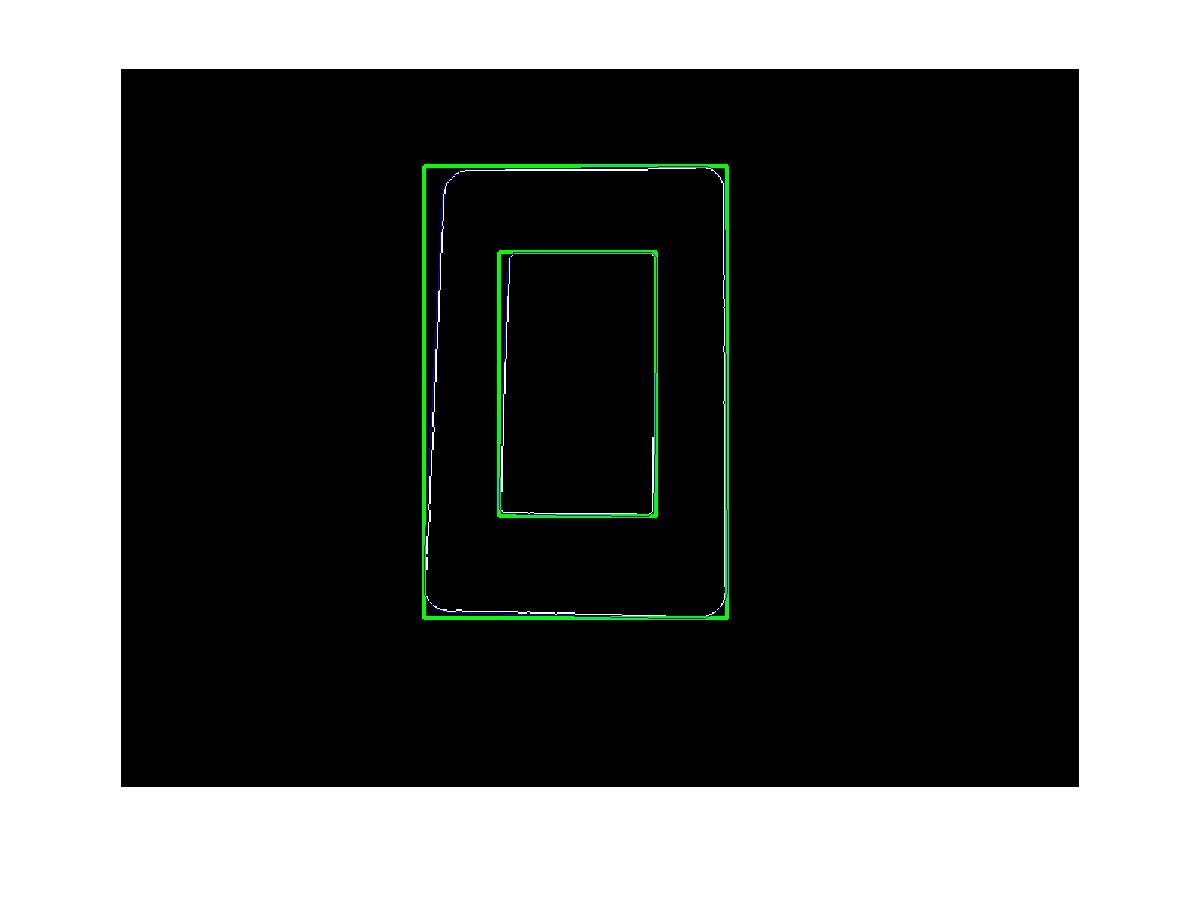
\includegraphics[scale=0.2]{convex_hull_main.jpg}
\end{center}
% \newline
\subsection{Thresholding the Features}
Before thresholding the features the histograms 
we inspected the histograms and by a method of trial and error we devised the location of the suits within the cropped card and tweaked the 
findthresh.m algorithm to target the correct
valley. It is important to note that our gray
intensity is conveniently between 0 and 1 due to a witty cast. The histograms were smoothed before iteration over then and as we went through the project:
\begin{center}
        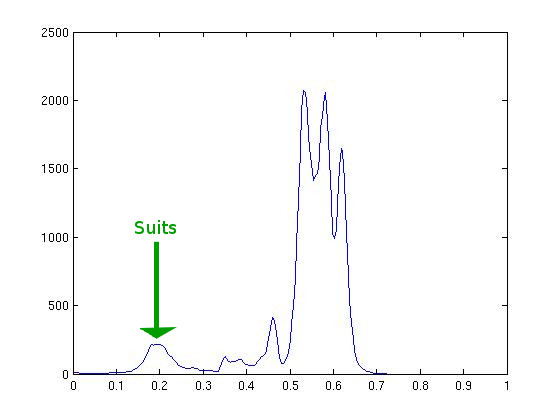
\includegraphics[scale=0.7]{suit.jpg}
\end{center}
The tiny peaks within a bigger peak were sources of distortion and mis-calibration thus we increased the size of the Gaussian kernel to blur these out more when convolving. Empirically we determined the kernel size to be 1x40 and it yielded histograms of the following form:
% \newline\newline
\begin{center}
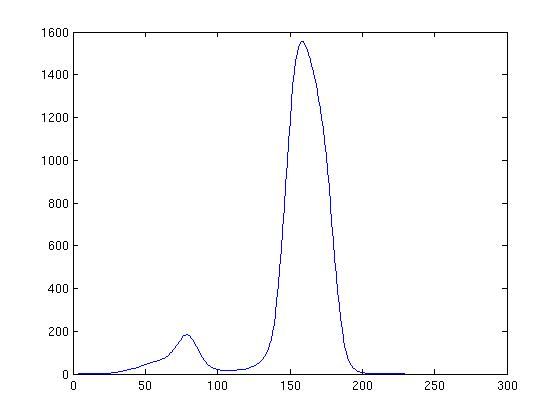
\includegraphics[scale=0.6]{histogram2.jpg}
\end{center}

After thresholding we removed small area (less than 150 px) elements and used the following morphological transform.  
\begin{lstlisting}
bw = bwmorph(bw,'mayority');
\end{lstlisting}
An additional noise removal technique (for long rectangles) was to look at the mayor axis to minor axis ratio and check that
it is not greater than 3. If it was greater than 3 we removed it. All these constants for removal were determined empirically
throughout the practical.
\begin{center}
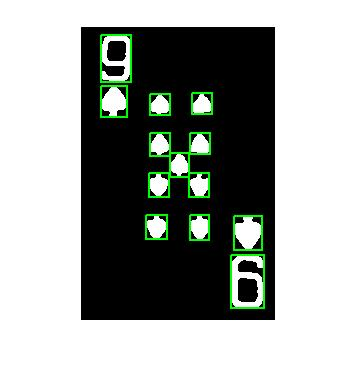
\includegraphics[scale=0.5]{properties.jpg}
\end{center}
We then found the bounding boxes for the remaining elements and cropped the original image (gray scaled) for each single one of these features. On every new cropped feature the following was applied to threshold
\begin{lstlisting}[mathescape]
% Inverted global threshold 
% graytrhesh computes global
% threshold level.
% we invert this to extract the suit
bw = $\text{\texttildelow}$im2bw(Icropped,graytrhesh(I));
\end{lstlisting}
resulting in: 
\begin{center}
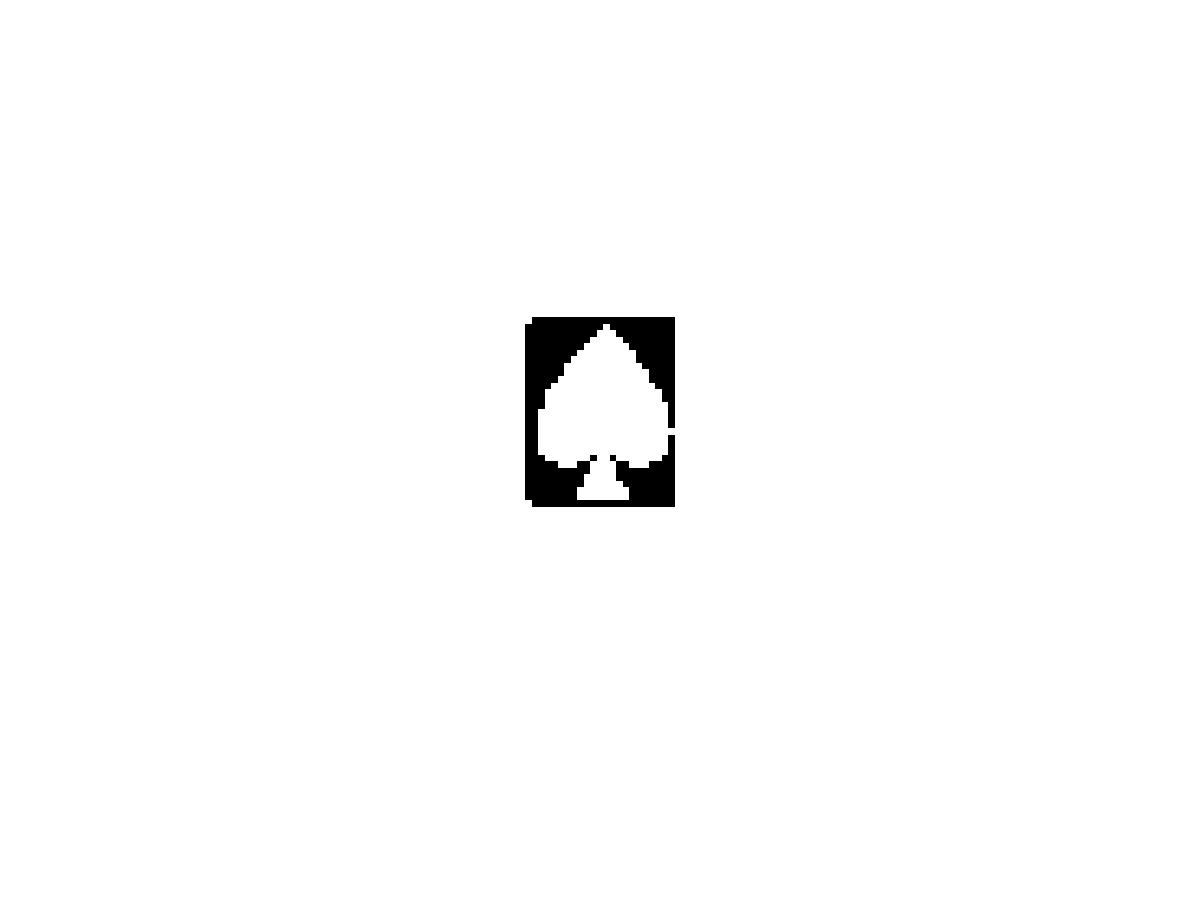
\includegraphics[scale=0.09]{spade_small.jpg}
\end{center}
This result was passed to getproperties.m to later generate the first 3 dimensions of our feature vector.
\subsection{Construction of Feature Vector for Suit classification}
For every suit symbol in each card we generated a feature vector. For example 2 of diamonds would ideally yield 4 feature vectors. The feature vectors consisted of 4 dimensions compactness, the first two rotation and scale invariant moments and the average of 
the normalized red channel of the suit which is closest to the center. The reasoning behind this is that the region detected closest to the center should be a suit (which yields a lot more pixels with color than a number); The closer you are to the center of the card the less likely the region is noise (again this is based on empirical evidence but also some common sense).
\[
\underline{x}_{feature} = \braket{\enskip compactness, \enskip ci_{1}, \enskip ci_{2}, \enskip \text{\bf mean}(red\_channel) \enskip}
\]
The other $ci_{k}, \enskip k \in [3,7]$ yield significantly small values along the order of magnitude of $10^{-5}$ and produced no changes in the classification problem, hence they were discarded due to their poor discrimination power. The normalization of the red channel before averaging accounts for dealing with brightness. We chose not to build two different classifiers since it seems quite hacky to identify red and black by assuming there normalized rgb values are approximately 0.3333 and 0.6 (which they are nonetheless when averaging within the bounding box of the suits these values may be averaged out resulting in confusion). 

\subsection{Complex Moments Disambiguation}
Black box approaches to using metrics are far from ideal and thus I have decided to disambiguate the complex moments since they originally seemed rather mysterious.
Moments are particular weighted averages used to describe image segments. The continuous version is :
\[c_{uv} =
\int^{\infty}_{-\infty}\int^{\infty}_{-\infty}(x -\mu_{x})^{u}(y - \mu_{y})^{v}dxdy
\]
If a particular image is rotated it experiences
the following linear transformation:

\[
\underline{x'}=
\begin{bmatrix}
  cos(\theta) & sin(\theta) \\
  -sin(\theta) & cos(\theta)  \\
 \end{bmatrix} \underline{x}
\]

for every $\underline{x}$ pixel in the image. In order to counteract the scale invariance one needs to counteract such linear transform with its inverse (since it is orthogonal that would just be its transpose):
\[
\underline{x}=
\begin{bmatrix}
  cos(\theta) & -sin(\theta) \\
  sin(\theta) & cos(\theta)  \\
 \end{bmatrix} \underline{x'}
\]
Having $\underline{x}$ we could just compute the regular moments invariant to rotation. Sadly determining $\theta$ is a tricky problem. One could find the principal components and estimate theta or use complex moments in the following manner:
\[
x = cos(\theta)x' - sin(\theta)y'
\]
\[
y = sin(\theta)x' + cos(\theta)y'
\]
Examining the following identity:
\[
z = a + ib 
\]
\[
z = r(cos(\theta) + isin(\theta))
\]
where $r = a^{2}+b^{2}$ one can observe the similarity between our desired linear transformations and complex numbers.
Thus 
\[
\int^{\infty}_{-\infty}\int^{\infty}_{-\infty}((x -\mu_{x})+(y - \mu_{y})i)^{u}((x -\mu_{x})-(y - \mu_{y})i)^{v}dxdy
\]
is a reasonable framework/approximation for:
\[
\int^{\infty}_{-\infty}\int^{\infty}_{-\infty}((x -\mu_{x})cos(\theta)+(y - \mu_{y})sin(\theta))^{u}((x -\mu_{x})cos(\theta)-(y - \mu_{y})sin(\theta))^{v}dxdy
\]
For the discrete case we just change integrals
to sums and sum over width and height.

\subsection{Counting the Number}
Out of 480 features (+ approximately 30 incorporated later) the detection of the features was perfect it drew the bounding box  on all features and no noise created any issues. This fact lead us to deciding that counting the number of regions and subtracting 4 was the correct decision for determining the number of the card. We opted out of naive Bayes since it is almost impossible to differentiate between 9 an 6 since they are exactly the same. A possible solution to classification via machine learning would be to compute the global moments of the card and incorporate them as dimensions since the 6 has less symbols than 9 the global moments and other global signatures could have relatively high discrimination powers.
\section{Results}
\subsection{Original Results}
The following results were obtained from the original 32 test cards provided.
\newline
\newline
{\bf Suits confusion matrix}
\newline
For the following results the precision per class and accuracy all yield 100\%.
 \begin{center}
    \begin{tabular}{| l | l |  l | l | p{2cm} |}
    \hline
      & spades & hearts & clubs &diamonds \\ \hline
 	   spades & 8 & 0 & 0 &0\\ \hline
 	   hearts & 0 & 8 & 0 &0\\ \hline
 	   clubs & 0 & 0 & 8 &0\\ \hline
 	   diamonds & 0 & 0 & 0&8\\ \hline
    \end{tabular}
 \end{center}
% \newline
% \newline
{\bf Numbers confusion matrix}
\newline
For the following results the precision per class and accuracy all yield 100\%.
\begin{center}
    \begin{tabular}{| l | l |  l | l |  l | l |  l | l |p{1cm} |}
    \hline
      & {\bf2} & {\bf3} & {\bf4} &{\bf5} &{\bf6} &{\bf7}&{\bf8}&{\bf9}\\ \hline
 	   {\bf2} & 4 & 0 &0  & 0 & 0 &  0&0 &0\\ \hline
 	   {\bf3} & 0 & 4 &  0& 0 &0  & 0 &0 &0\\ \hline
 	   {\bf4} & 0 & 0 & 4 &  0& 0 &  0& 0&0\\ \hline
 	   {\bf5} & 0 & 0 & 0 & 4 &  0& 0 & 0&0\\ \hline
 	   {\bf6} & 0 & 0 & 0 & 0 &4  & 0 &0 &0\\ \hline
 	   {\bf7} & 0 & 0 & 0 & 0 & 0 &4  & 0&0\\ \hline
 	   {\bf8} & 0 & 0 & 0 & 0 & 0 &0  &4 &0\\ \hline
 	   {\bf9 }& 0 & 0 & 0 & 0 & 0 &0  &0 &4\\ \hline
    \end{tabular}
 \end{center}
 \newpage
{\bf Suits confusion matrix 240 features}
\newline
For the following results the precision of spades, clubs and hearts yield 100\% and overall accuracy :99.6\%. For diamonds precision is 98\%. 
 \begin{center}
    \begin{tabular}{| l | l |  l | l | p{2cm} |}
    \hline
      & spades & hearts & clubs &diamonds \\ \hline
 	   spades & 60 & 0 & 0 &0\\ \hline
 	   hearts & 0 & 60 & 0 &0\\ \hline
 	   clubs & 0 & 0 & 60 &0\\ \hline
 	   diamonds & 0 & 1 & 0&59\\ \hline
    \end{tabular}
 \end{center}
\subsection{Extra 8 Cards}
Several new cards were added in addition. They all experienced transformations such as increase and decrease in brightness, rotation, contrast and perspective.
\newline
\newline
{\bf Suits confusion matrix}
\newline
For the following results the precision per class and accuracy all yield 100\%.
 \begin{center}
    \begin{tabular}{| l | l |  l | l | p{2cm} |}
    \hline
      & spades & hearts & clubs &diamonds \\ \hline
 	   spades & 13 & 0 & 0 &0\\ \hline
 	   hearts & 0 & 11 & 0 &0\\ \hline
 	   clubs & 0 & 0 & 8 &0\\ \hline
 	   diamonds & 0 & 0 & 0&8\\ \hline
    \end{tabular}
 \end{center}
% \newline
% \newline
{\bf Numbers confusion matrix}
\newline
For the following results the precision per class and accuracy all yield 100\%.
\begin{center}
    \begin{tabular}{| l | l |  l | l |  l | l |  l | l |p{1cm} |}
    \hline
      & {\bf2} & {\bf3} & {\bf4} &{\bf5} &{\bf6} &{\bf7}&{\bf8}&{\bf9}\\ \hline
 	   {\bf2} & 9 & 0 &0  & 0 & 0 &  0&0 &0\\ \hline
 	   {\bf3} & 0 & 4 &  0& 0 &0  & 0 &0 &0\\ \hline
 	   {\bf4} & 0 & 0 & 4 &  0& 0 &  0& 0&0\\ \hline
 	   {\bf5} & 0 & 0 & 0 & 4 &  0& 0 & 0&0\\ \hline
 	   {\bf6} & 0 & 0 & 0 & 0 &5  & 0 &0 &0\\ \hline
 	   {\bf7} & 0 & 0 & 0 & 0 & 0 &4  & 0&0\\ \hline
 	   {\bf8} & 0 & 0 & 0 & 0 & 0 &0  &4 &0\\ \hline
 	   {\bf9 }& 0 & 0 & 0 & 0 & 0 &0  &0 &6\\ \hline
    \end{tabular}
 \end{center}
 \newpage
{\bf Suits confusion matrix 240 features}
\newline
For the following results the precision of spades and clubs yield 100\% and overall accuracy :98.96\%. For diamonds precision is 98.3\% and for diamonds precision is 97.7\%. 
 \begin{center}
    \begin{tabular}{| l | l |  l | l | p{2cm} |}
    \hline
      & spades & hearts & clubs &diamonds \\ \hline
 	   spades & 80 & 0 & 0 &0\\ \hline
 	   hearts & 0 & 88 & 2 &0\\ \hline
 	   clubs & 0 & 0 & 60 &0\\ \hline
 	   diamonds & 0 & 1 & 0&59\\ \hline
    \end{tabular}
 \end{center}
\subsection{First Batch of Results}
The following results were obtained from the original 32 test cards provided. In this trial we attempted normalization before thresholding. In the first place this was a bad idea since for black cards gray, black and white all become more or less the same value. Secondly matlab did a strange double cast which corrupted the results of the normalization. After debugging and removing normalization results improved.
\newline
\newline
{\bf Suits confusion matrix}
\newline
For the following results the precision per class and accuracy all yield 100\%.
 \begin{center}
    \begin{tabular}{| l | l |  l | l | p{2cm} |}
    \hline
      & spades & hearts & clubs &diamonds \\ \hline
 	   spades & 8 & 0 & 0 &0\\ \hline
 	   hearts & 0 & 8 & 0 &0\\ \hline
 	   clubs & 0 & 0 & 8 &0\\ \hline
 	   diamonds & 0 & 0 & 0&8\\ \hline
    \end{tabular}
 \end{center}
% \newline
% \newline
{\bf Numbers confusion matrix}
\newline
For the following results the precision per class and accuracy all yield 100\%.
\begin{center}
    \begin{tabular}{| l | l |  l | l |  l | l |  l | l |p{1cm} |}
    \hline
      & {\bf2} & {\bf3} & {\bf4} &{\bf5} &{\bf6} &{\bf7}&{\bf8}&{\bf9}\\ \hline
 	   {\bf2} & 4 & 0 &0  & 0 & 0 &  0&0 &0\\ \hline
 	   {\bf3} & 0 & 4 &  0& 0 &0  & 0 &0 &0\\ \hline
 	   {\bf4} & 0 & 0 & 4 &  0& 0 &  0& 0&0\\ \hline
 	   {\bf5} & 0 & 0 & 0 & 4 &  0& 0 & 0&0\\ \hline
 	   {\bf6} & 0 & 0 & 0 & 0 &4  & 0 &0 &0\\ \hline
 	   {\bf7} & 0 & 0 & 0 & 0 & 0 &4  & 0&0\\ \hline
 	   {\bf8} & 0 & 0 & 0 & 0 & 0 &0  &4 &0\\ \hline
 	   {\bf9 }& 0 & 0 & 0 & 0 & 0 &0  &0 &4\\ \hline
    \end{tabular}
 \end{center}
 \newpage
{\bf Suits confusion matrix 240 features}
\newline
\newline
For the following results the precision of spades and hearts yield 100\% and overall accuracy :98.3\%. For clubs precision is 96.7\% and for diamonds precision is 96.7\%.
 \begin{center}
    \begin{tabular}{| l | l |  l | l | p{2cm} |}
    \hline
      & spades & hearts & clubs &diamonds \\ \hline
 	   spades & 60 & 0 & 0 &0\\ \hline
 	   hearts & 0 & 60 & 0 &0\\ \hline
 	   clubs & 2 & 0 & 58 &0\\ \hline
 	   diamonds & 0 & 2 & 0&58\\ \hline
    \end{tabular}
 \end{center}

 \subsection{Extreme Experiments}
 All of the following experiments classified the cards correctly:
 \newline
 {\bf Drawn Card on Wooden Background}
 \newline
 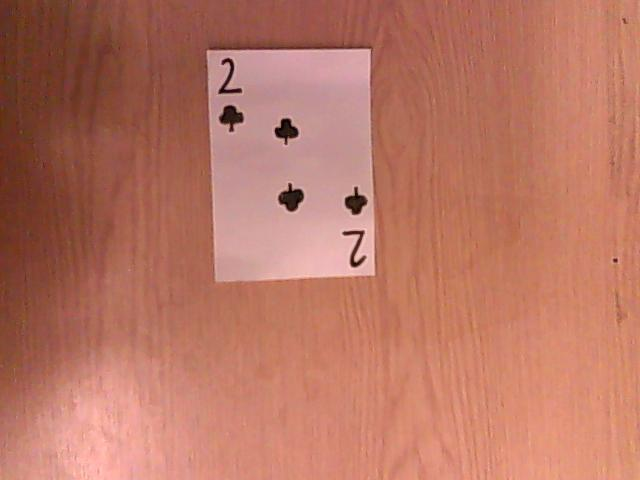
\includegraphics[scale=0.1]{test0.jpg}
  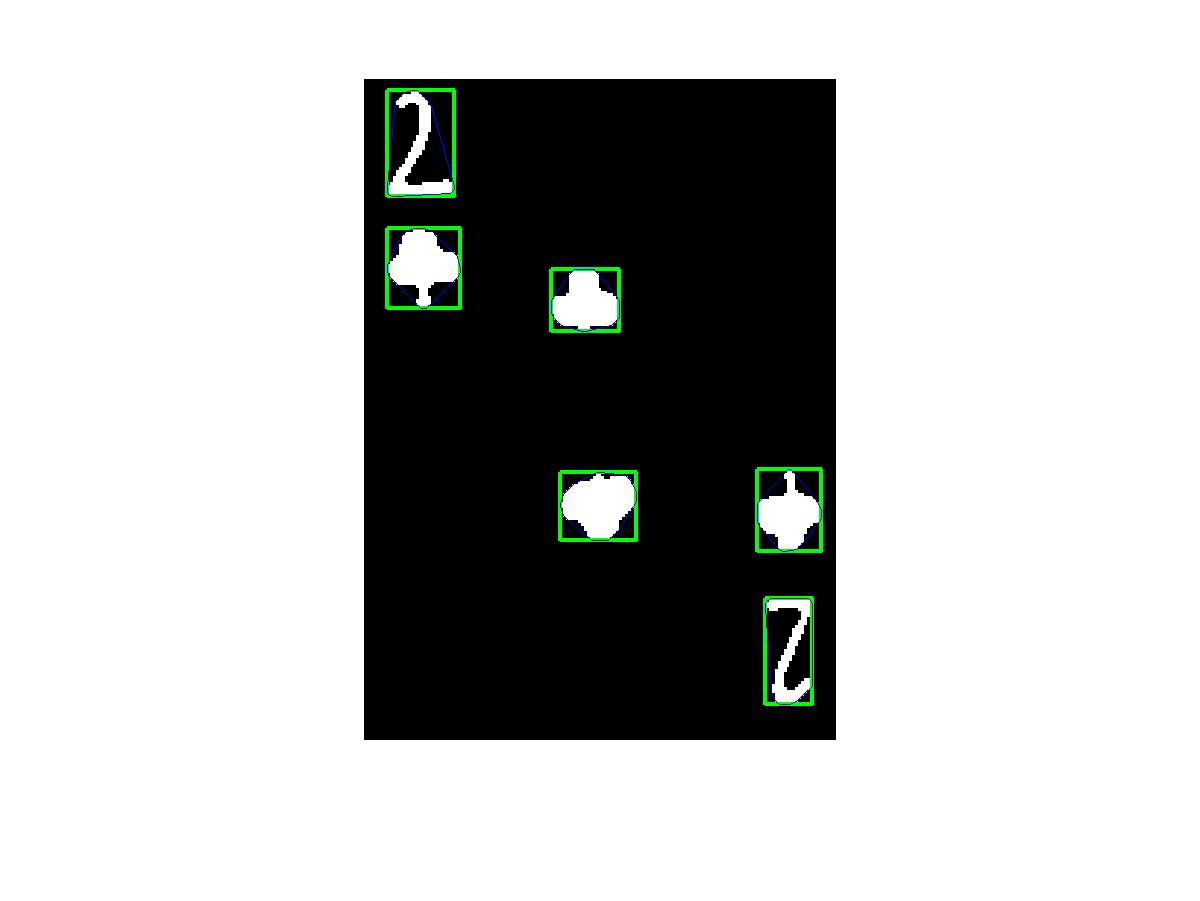
\includegraphics[scale=0.07]{paperfull.jpg}
  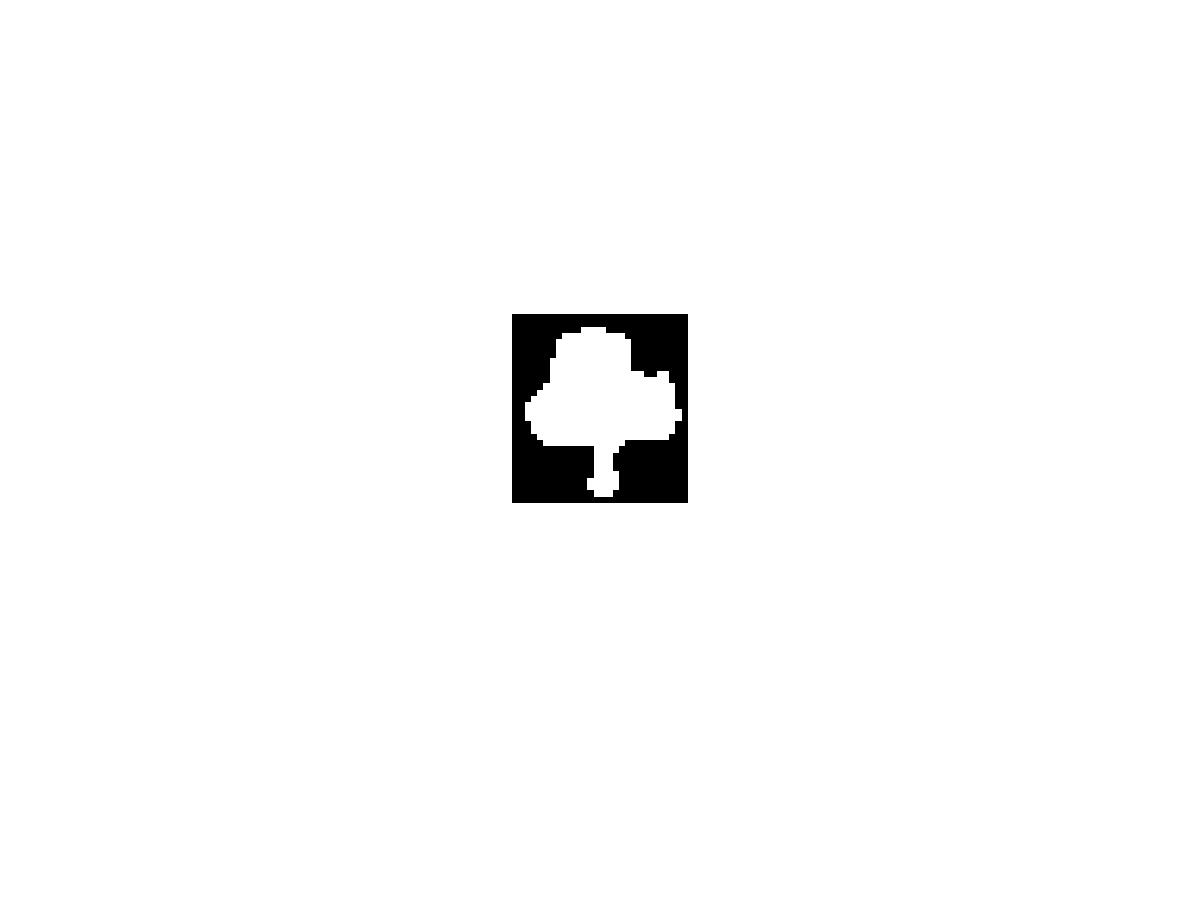
\includegraphics[scale=0.07]{paperfeat.jpg}
  \newline
 {\bf Horizontal Card}
 \newline
 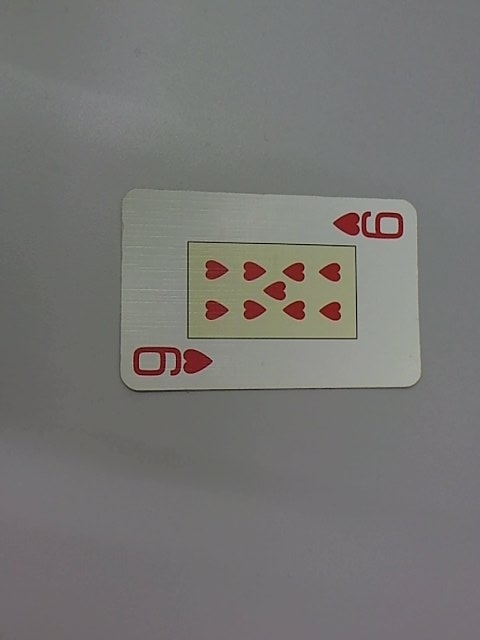
\includegraphics[scale=0.1]{test2_90.jpg}
  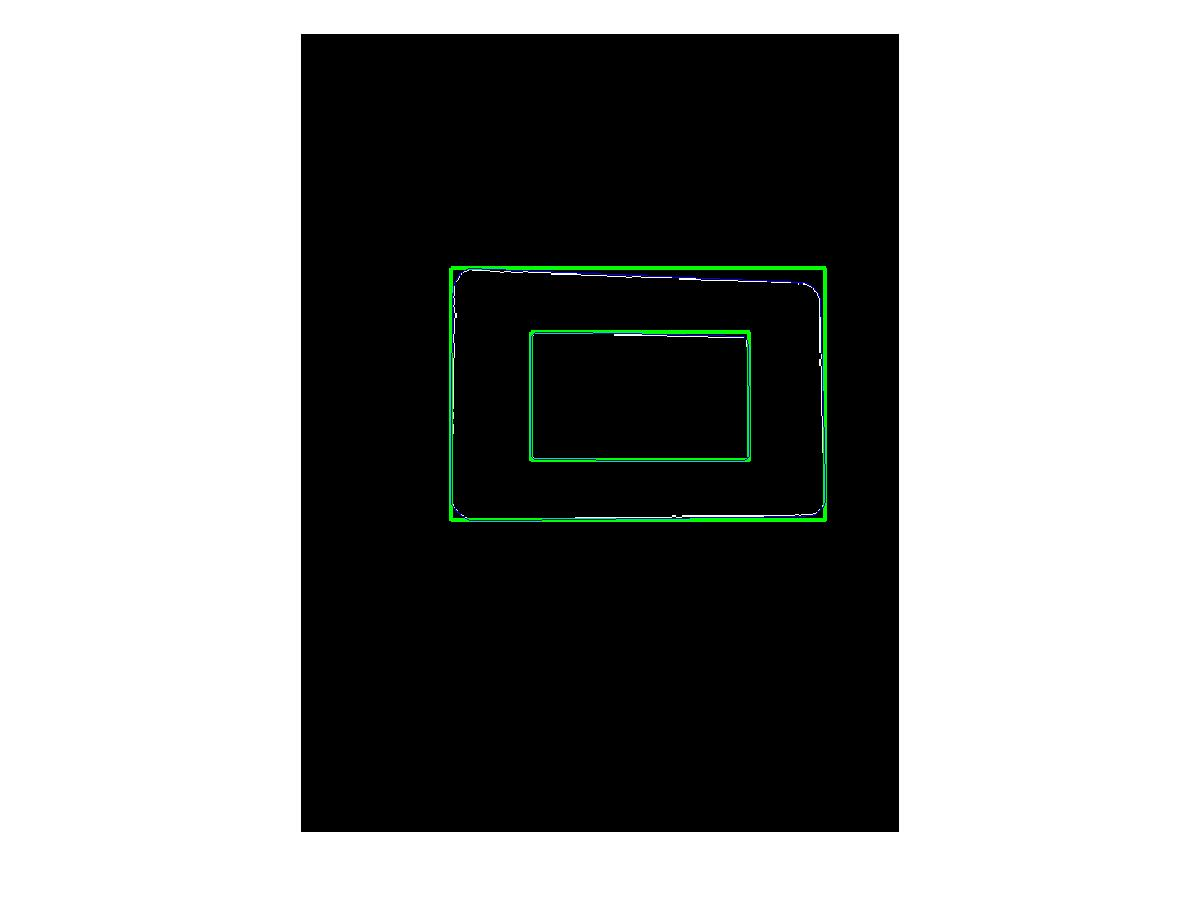
\includegraphics[scale=0.07]{rotated_main.jpg}
  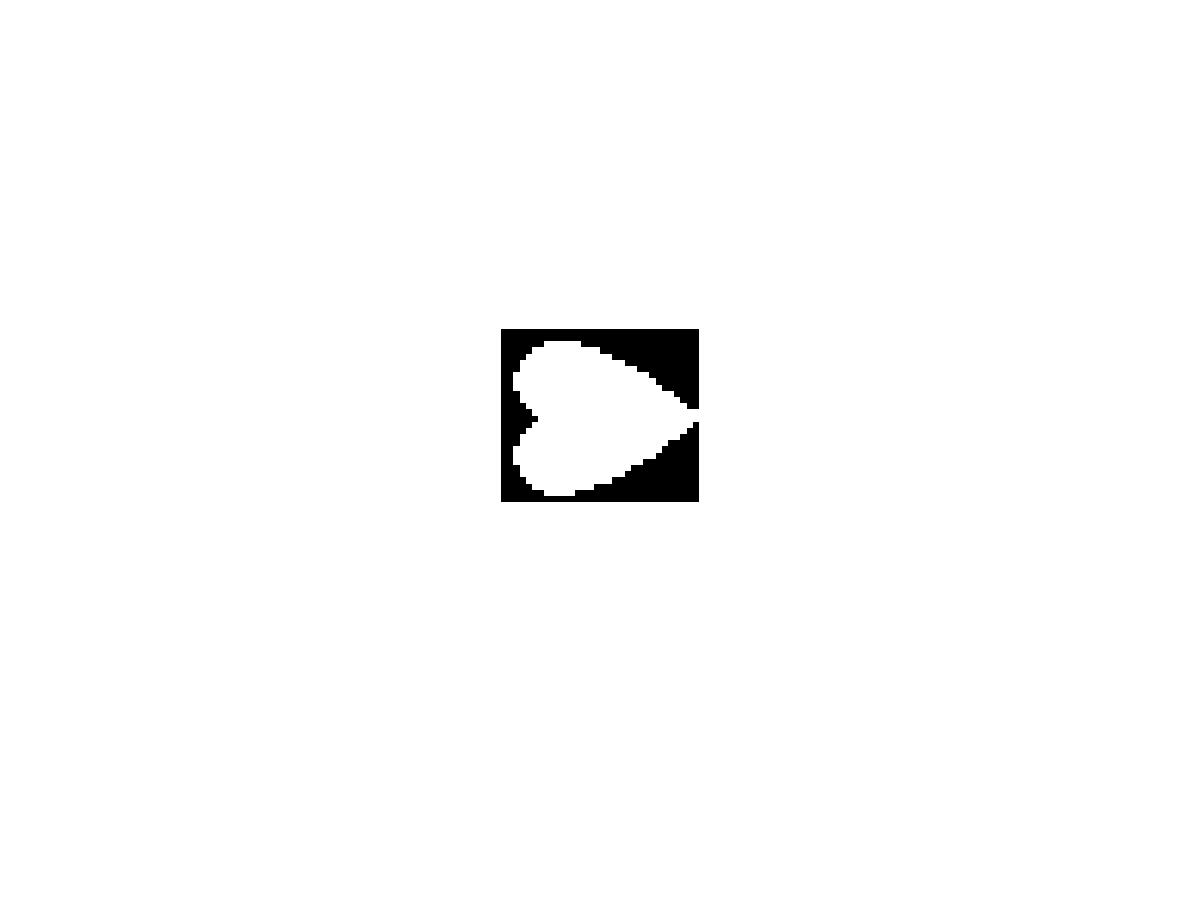
\includegraphics[scale=0.07]{rotated_heart.jpg}
  \newline
   {\bf Angled Card}
 \newline
 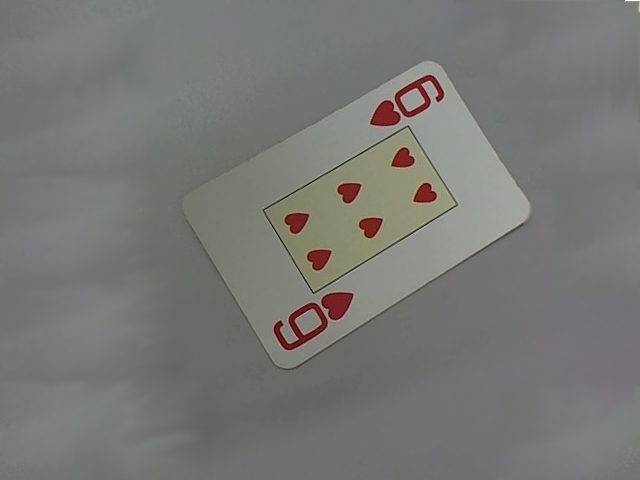
\includegraphics[scale=0.1]{train18_1.jpg}
  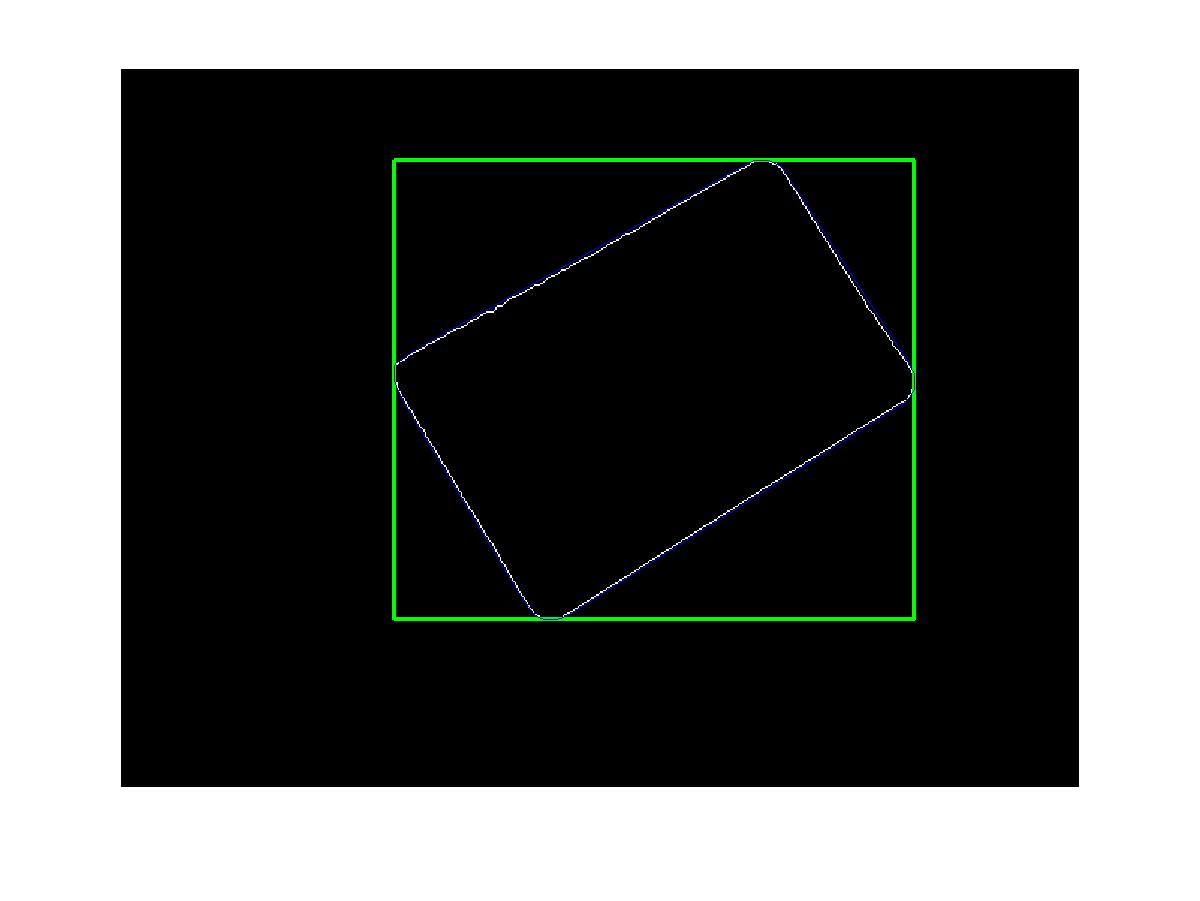
\includegraphics[scale=0.07]{rotated_some_6_main.jpg}
  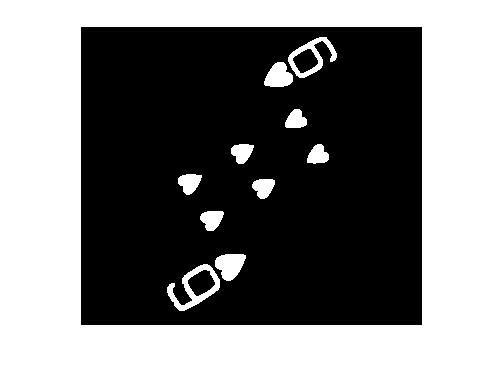
\includegraphics[scale=0.2]{rotate_works.jpg}
  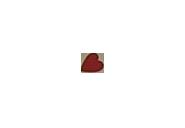
\includegraphics[scale=0.4]{rotate2.jpg}
% \subsecion{}
\end{document}